\documentclass{standalone}
\usepackage{tikz}
\usetikzlibrary{shapes.geometric, positioning, arrows.meta}
\usepackage{palatino} % Use the Palatino font

\begin{document}
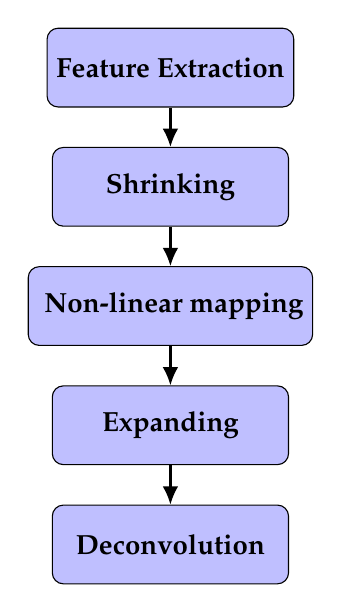
\begin{tikzpicture}[
  node distance=0.5cm and 0cm,
  every node/.style={draw, rounded corners, align=center},
  parent_class/.style={rectangle, minimum width=3cm, minimum height=1cm, fill=blue!25},
  class/.style={rectangle, minimum width=3cm, minimum height=1cm, fill=blue!25},
  implementation/.style={rectangle, minimum width=3cm, minimum height=0.25cm, fill=green!25},
  arrow/.style={-{Latex[width=2mm]}, thick}
]

% Classes
\node[parent_class] (experiment) {\textbf{Feature Extraction}};
\node[class] (s1) [below =of experiment] {\textbf{Shrinking}};
\node[class] (s2) [below =of s1] {\textbf{ Non-linear mapping}};
\node[class] (s3) [below =of s2] {\textbf{Expanding}};
\node[class] (s4) [below =of s3] {\textbf{Deconvolution}};


% Experiment connections
% \draw[arrow] (experiment) -- (model);
\draw[arrow] (experiment) -- (s1);
\draw[arrow] (s1) -- (s2);
\draw[arrow] (s2) -- (s3);
\draw[arrow] (s3) -- (s4);


% % Experiment implementations
% \node[implementation] (experiment1) [below=of experiment] {{Feature Extraction}};
% \node[implementation] (experiment2) [below=of experiment1] {{Shrinking}};
% \node[implementation] (experiment3) [below=of experiment2] {{Non-linear mapping}};
% \node[implementation] (experiment4) [below=of experiment3] {{Expanding}};
% \node[implementation] (experiment5) [below=of experiment4] {{Deconvolution}};


% Model Implementations
% \node[implementation] (model1) [below=of model] {{Ridge Regression}};
% \node[implementation] (model2) [below=of model1] {{XGBoost}};
% \node[implementation] (model3) [below=of model2] {{Neural Net}};

% % Data Implementations
% \node[implementation] (data1) [below=of data] {{Baseline Data}};
% \node[implementation] (data2) [below=of data1] {{Extended Data}};

% Draw arrows for implementations
% \draw[arrow] (model) -- (model1);
% \draw[arrow] (model) -- (model2);
% \draw[arrow] (model) -- (model3);

% \draw[arrow] (data) -- (data1);
% \draw[arrow] (data) -- (data2);

% Title
% \node[draw=none, fill=none] (title) [above=of experiment] {Metodología Experimental};

\end{tikzpicture}
\end{document}
